\documentclass[a4paper]{article}
\usepackage[utf8]{inputenc}
\usepackage[russian]{babel}
\usepackage[T2A]{fontenc}
\usepackage[warn]{mathtext}
\usepackage{graphicx}
\usepackage{floatflt}
\usepackage[left=30mm, top=20mm, right=20mm, bottom=20mm, footskip=10mm]{geometry}
\usepackage{multirow}
\usepackage{amsmath}

\graphicspath{ {./images/} }
\usepackage{multicol}
\setlength{\columnsep}{2cm}

\begin{document}

\begin{titlepage}
	\centering
	{\scshape\Large Mосковский физико-технический институт \\ (национальный исследовательский университет) \par}
	\vspace{6cm}
	{\scshape\Large Отчет о выполнении лабораторной работы 2.2.5 \par}
	\vspace{1cm}
	{\huge\bfseries Определение вязкости жидкости по скорости истечения через капилляр \par}
	\vspace{4cm}
	\vfill
	\begin{flushright}
		{\large Выполнил: \\ Градовцев Святослав Алексеевич \\ Б03-504 \par}
	\end{flushright}
	\vfill
	{\large \centering Долгопрудный 2026 \par}
\end{titlepage}

\section{Цель работы}
\begin{enumerate}
    \item определение вязкости воды по измерению объёма жидкости, протёкшей через капилляр
    \item определение вязкости других жидкостей путём сравнения скорости их перетекания со скоростью перетекания воды
\end{enumerate}

\section{В работе используются}
\begin{itemize}
    \item сосуд Мариотта
    \item капиллярная трубка
    \item мензурка
    \item секундомер
    \item стакан
    \item микроскоп на стойке
\end{itemize}

\section{Измерение вязкости воды}
\subsection{Теоретические положения}
Формула Пуазейля для расхода жидкости через сечение трубки:
$$Q = \pi \frac{P_1-P_2}{8 \eta l} R^4$$

Число Рейнольдса:
$$Re = \frac{v R \rho}{\eta}$$

В гладких трубах круглого сечения переход от ламинарного движения к турбулентному происходит при $Re \approx 1000$.

Ламинарное движение жидкости при переходе ее из широкого сосуда в капилляр устанавливается не сразу, а после прохождения расстояния $a$:
$$a \approx 0,2R \cdot Re$$

\subsection{Экспериментальная установка}
\begin{figure}[h]
    \centering
    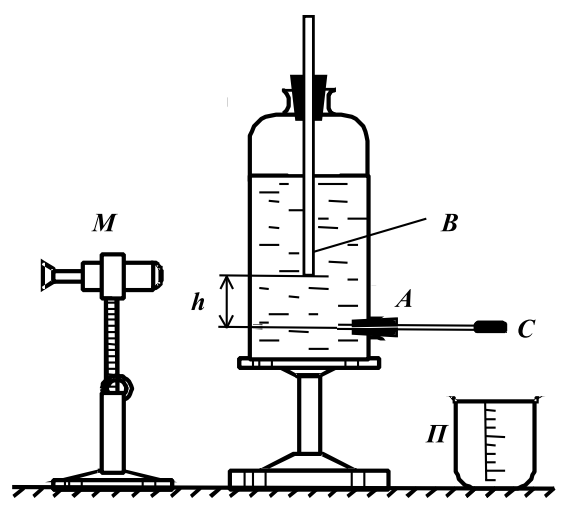
\includegraphics[width=7cm]{setup1.PNG}
    \caption{Схема установки для определения вязкости воды}
    \label{fig:vac}
\end{figure}

\subsection{Ход работы}
\begin{enumerate}
    \item Измерение геометрических параметров капилляра.
    \begin{itemize}
        \item Длина капилляра: $l = 135 \pm 1$ мм.
        \item Измерение диаметра капилляра. Результаты представлены в таблице 1. Инструментальная погрешность $\sigma_{D,\text{инстр}} = 0,025$ мм.
    \end{itemize}

    \begin{table}[h]
        \centering
        \caption{Измерение диаметра капилляра}
        \label{tab:diam}
        \begin{tabular}{|c|c|}
        \hline
        Номер измерения & $D_i$, мм \\
        \hline
        1 & 0,375 \\
        2 & 0,400 \\
        3 & 0,375 \\
        4 & 0,375 \\
        \hline
        \end{tabular}
    \end{table}

    Среднее значение диаметра: $\bar D = 0,381$ мм. \\
    Случайная погрешность: $\sigma_{D,\text{случ}} = 0,006$ мм. \\
    Полная погрешность: $\sigma_D = \sqrt{0,006^2 + 0,025^2} = 0,026$ мм. \\
    Диаметр капилляра: $D = (0,381 \pm 0,026)$ мм. \\
    Радиус капилляра: $R = D/2 = 0,191$ мм. Погрешность радиуса: $\sigma_R = 0,013$ мм.

    \item Определение поправки $\Delta h$, обусловленной силами поверхностного натяжения.
    $$\Delta h = (9,50 \pm 0,03)\ \text{мм}$$

    \item Измерение расхода воды при различных значениях $h$. Результаты занесены в таблицу 2. Объём истекшей жидкости $V = 20,0 \pm 0,05$ см$^3$. Погрешность времени $\sigma_{t,\text{пр}} = 0,01$ с.

    \begin{table}[h]
        \centering
        \caption{Зависимость расхода воды от перепада давлений}
        \label{tab:marriott}
        \begin{tabular}{|c|c|c|}
        \hline
        $h$, мм & $t$, с & $Q = V/t$, см$^3$/с \\
        \hline
        26,1 & $950,00 \pm 0,01$ & 0,0211 \\
        36,7 & $696,00 \pm 0,01$ & 0,0287 \\
        48,0 & $540,00 \pm 0,01$ & 0,0370 \\
        65,5 & $375,00 \pm 0,01$ & 0,0533 \\
        \hline
        \end{tabular}
    \end{table}

    Для проверки ламинарности течения рассчитаем число Рейнольдса, приняв $\eta \approx 0,01$ Пуаз.
    
    \begin{center}
    \begin{tabular}{|c|c|c|}
    \hline
    $Q$, см$^3$/с & $Re$ & $a$, мм \\
    \hline
    0,0211 & 70 & 2,7 \\
    0,0287 & 96 & 3,7 \\
    0,0370 & 124 & 4,7 \\
    0,0533 & 178 & 6,8 \\
    \hline
    \end{tabular}
    \end{center}
    
    Во всех опытах $Re < 1000$, течение ламинарное. Длина капилляра $l = 135$ мм значительно больше $a$, поэтому формула Пуазейля применима.

    \item Построим график зависимости $Q(h)$ (рис. 2). Согласно формуле Пуазейля, $Q = \frac{\pi R^4 \rho g}{8 \eta l} (h - \Delta h)$, зависимость линейна. Экстраполяция прямой на ось $h$ при $Q=0$ даёт $\Delta h_{\text{граф}} \approx 9.1$ мм.

    \begin{figure}[t]
        \centering
        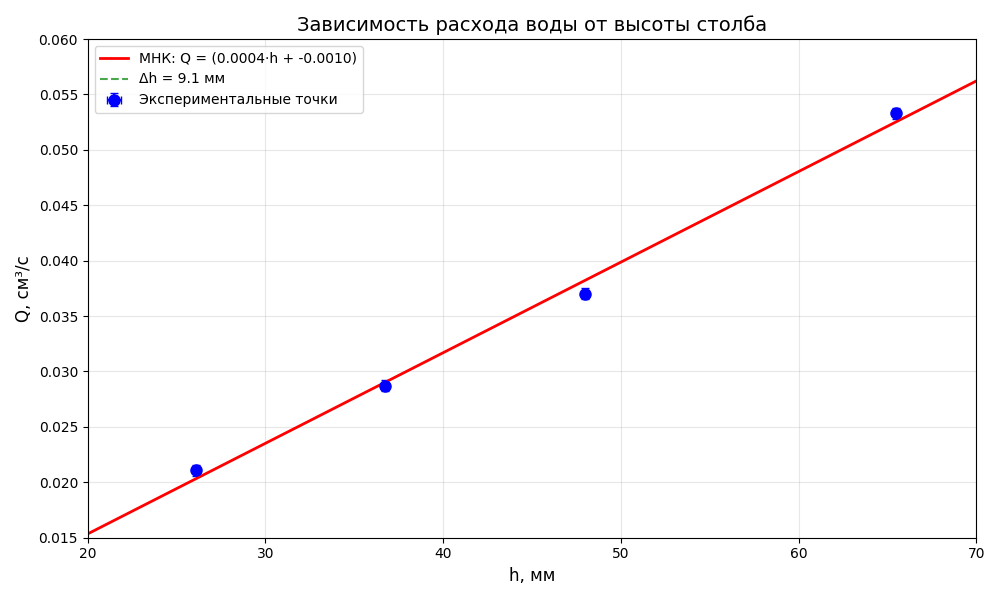
\includegraphics[width=\textwidth]{graph1.PNG}
        \caption{График зависимости расхода воды от высоты столба}
        \label{fig:graph1}
    \end{figure}

    По углу наклона прямой определяем вязкость воды:
    $$\eta = \frac{\pi R^4 \rho g}{8 l} \cdot \left(\frac{dQ}{dh}\right)^{-1} = 0,00896\ \text{Пуаз}.$$

    Погрешность:
    \begin{center}
    $\sigma \eta = \eta \sqrt{(\frac{\sigma h}{h})^2 + 4^2(\frac{\sigma R}{R})^2 + (\frac{\sigma l}{l})^2} = 0,0025$ П
    \end{center}

    Табличное значение вязкости воды при $25^\circ C$: $\eta_{\text{табл}} = 0,00891$ Пуаз. Экспериментальное значение в пределах погрешности совпадает с табличным.

    \begin{center}
    \fbox{$\eta_{\text{табл}} = 0,00891$ Пуаз \hspace{1cm} $\eta_{\text{эксп}} = 0,0090 \pm 0,0025$ Пуаз}
    \end{center}
\end{enumerate}

\section{Измерение вязкости водного раствора глицерина вискозиметром Оствальда}
\subsection{Теоретические положения}
Для вискозиметра Оствальда:
$$\frac{\rho_1}{\eta_1}t_1 = \frac{\rho_2}{\eta_2}t_2 = const$$

Рабочая формула:
$$\eta_x = \eta_0\frac{\rho_x}{\rho_0}\frac{t_x}{t_0}$$


\subsection{Ход работы}
\begin{enumerate}
    \item Измерение времени истечения жидкостей. Результаты приведены в таблице 3. Приборная погрешность секундомера $\sigma_{t,\text{пр}} = 0,01$ с.

    \begin{table}[h]
        \centering
        \caption{Время протекания жидкостей между метками вискозиметра}
        \label{tab:ostwald}
        \begin{tabular}{|c|c|c|c|}
        \hline
        \multirow{2}{*}{Вещество} & \multirow{2}{*}{Плотность, г/см$^3$} & \multicolumn{2}{c|}{Время истечения} \\ \cline{3-4}
         & & $t_i$, с & $\bar t \pm \sigma_t$, с \\
        \hline
        \multirow{3}{*}{Вода} & \multirow{3}{*}{0,997} & 9,33 & \multirow{3}{*}{$9,37 \pm 0,03$} \\
         & & 9,37 & \\
         & & 9,42 & \\
        \hline
        \multirow{3}{*}{Глицерин 10\%} & \multirow{3}{*}{1,019} & 12,64 & \multirow{3}{*}{$12,68 \pm 0,04$} \\
         & & 12,76 & \\
         & & 12,65 & \\
        \hline
        \multirow{3}{*}{Глицерин 20\%} & \multirow{3}{*}{1,042} & 16,12 & \multirow{3}{*}{$16,25 \pm 0,07$} \\
         & & 16,37 & \\
         & & 16,27 & \\
        \hline
        \multirow{3}{*}{Глицерин 30\%} & \multirow{3}{*}{1,065} & 19,34 & \multirow{3}{*}{$19,36 \pm 0,02$} \\
         & & 19,36 & \\
         & & 19,39 & \\
        \hline
        \end{tabular}
    \end{table}

    \item Расчёт вязкости растворов глицерина:
    
    $$\eta_x = \eta_0\frac{\rho_x}{\rho_0}\frac{t_x}{t_0}, \quad 
    \sigma_{\eta_x} = \eta_x \sqrt{\left(\frac{\sigma_{\eta_0}}{\eta_0}\right)^2 + \left(\frac{\sigma_{t_x}}{t_x}\right)^2 + \left(\frac{\sigma_{t_0}}{t_0}\right)^2}$$
    
    где $\eta_0 = 0,00896$ Пуаз — вязкость воды из первой части работы.

    Полученные значения (в сантипуазах):
    
    $$\eta_{10} = 1,24\ \text{сП}, \quad \sigma_{\eta_{10}} = 0,4\ \text{сП}$$
    $$\eta_{20} = 1,62\ \text{сП}, \quad \sigma_{\eta_{20}} = 0,5\ \text{сП}$$
    $$\eta_{30} = 1,97\ \text{сП}, \quad \sigma_{\eta_{30}} = 0,6\ \text{сП}$$

    Сравнение с табличными значениями представлено в таблице 4.

    \begin{table}[h]
        \centering
        \caption{Сравнение экспериментальных и табличных значений вязкости}
        \label{tab:compare}
        \begin{tabular}{|c|c|c|}
        \hline
        Раствор & $\eta_{\text{эксп}}$, сП & $\eta_{\text{табл}}$, сП \\
        \hline
        10\% глицерин & $1,24 \pm 0,4$ & 1,31 \\
        20\% глицерин & $1,62 \pm 0,5$ & 1,76 \\
        30\% глицерин & $1,97 \pm 0,6$ & 2,31 \\
        \hline
        \end{tabular}
    \end{table}
\end{enumerate}

\section{Вывод}
В ходе работы были определены вязкости воды и водных растворов глицерина.
\begin{enumerate}
    \item Вязкость воды, измеренная абсолютным методом, составила $\eta = (0,0090 \pm 0,0025)$ Пуаз, что согласуется с табличным значением $0,00891$ Пуаз.
    \item Вязкости растворов глицерина:
    \begin{itemize}
        \item 10\%: $\eta = 1,24 \pm 0,4$ сП
        \item 20\%: $\eta = 1,62 \pm 0,5$ сП
        \item 30\%: $\eta = 1,97 \pm 0,6$ сП
    \end{itemize}
    Результаты для 10\% и 20\% растворов попадают в интервал погрешности табличных данных.
\end{enumerate}

\end{document}